\documentclass{beamer}

%%%%%%%%%%%%%%%%%%%%%%%%%%%%%%%%%%%%%%%%%%%%%%%%%%%%%%%%%%%%%%%%
%%%                  Themes and such                         %%%
%%%%%%%%%%%%%%%%%%%%%%%%%%%%%%%%%%%%%%%%%%%%%%%%%%%%%%%%%%%%%%%%
\mode<presentation>
{
%  \usetheme{Copenhagen}  
  \usetheme{Warsaw}  
%  \usetheme{Malmoe}  

  %make my huge toc fit on one slide (and not look horrible)
  \setbeamerfont{subsection in toc}{series=\bfseries}
  \setbeamerfont{subsection in toc}{size=\tiny,series=\bfseries}
}
%\setbeamersize{text margin left=0.5cm,text margin right=0.5cm}

%%%%%%%%%%%%%%%%%%%%%%%%%%%%%%%%%%%%%%%%%%%%%%%%%%%%%%%%%%%%%%%%
%%%                       Packages                           %%%
%%%%%%%%%%%%%%%%%%%%%%%%%%%%%%%%%%%%%%%%%%%%%%%%%%%%%%%%%%%%%%%%
\usepackage{multimedia}
\usepackage{multirow}


% Define commands 

 \newcommand{\half}{\ensuremath{\frac{1}{2}}}

 \newcommand{\bea}{\begin{eqnarray}}
 \newcommand{\eea}{\end{eqnarray}}
 \newcommand{\beq}{\begin{equation}}
 \newcommand{\eeq}{\end{equation}}
 \newcommand{\bed}{\begin{displaymath}}
 \newcommand{\eed}{\end{displaymath}}
\newcommand{\pd}[2]{\frac{\partial #1}{\partial #2}}
\newcommand{\pf}[2]{\frac{d #1}{d #2}}
\newcommand{\pdt}[2]{\frac{\partial^2 #1}{\partial #2^2}}
\newcommand{\pft}[2]{\frac{d^2 #1}{d #2^2}}
\newcommand{\pdtno}[2]{\frac{\partial^2 #1}{\partial #2}}
\newcommand{\pdd}[3]{\frac{\partial^2 #1}{\partial #2 \partial #3}}
\newcommand{\pff}[3]{\frac{d^2 #1}{d #2 d #3}}

%%%%%%%%%%%%%%%%%%%%%%%%%%%%%%%%%%%%%%%%%%%%%%%%%%%%%%%%%%%%%%%%
%%%                     Title Info                           %%%
%%%%%%%%%%%%%%%%%%%%%%%%%%%%%%%%%%%%%%%%%%%%%%%%%%%%%%%%%%%%%%%%

\title[\hspace{-0.2cm} Isogeometric Analysis Using NURBS]
{
  Isogeometric Finite Element Analysis Using Non-uniform Rational Bsplines
}

\author[ME6104 Project, K. Boopathy, S. Niranjan Babu, April 2019]
{
  \large {Komahan Boopathy}\\
  \large Siddarth Niranjan Babu \\
}

\institute
{
  \Large {\textbf{ME6104 Computer Aided Design -- Final Project}} \\
  \vspace{0.2in}
  \large Georgia Institute of Technology\\
  School of Aerospace Engineering
}

\date
{
\small \today
}




%%%%%%%%%%%%%%%%%%%%%%%%%%%%%%%%%%%%%%%%%%%%%%%%%%%%%%%%%%%%%%%%
%%%                   Begin Document                         %%%
%%%%%%%%%%%%%%%%%%%%%%%%%%%%%%%%%%%%%%%%%%%%%%%%%%%%%%%%%%%%%%%%

\begin{document}

%%%%%%%%%%%%%%%%%%%%%%%%%%%%%%%%%%%%%%%%%%%%%%%%%%%%%%%%%%%%%%%%
%%%                     Title Page                           %%%
%%%%%%%%%%%%%%%%%%%%%%%%%%%%%%%%%%%%%%%%%%%%%%%%%%%%%%%%%%%%%%%%

\begin{frame}
  \titlepage
\end{frame}

%%%%%%%%%%%%%%%%%%%%%%%%%%%%%%%%%%%%%%%%%%%%%%%%%%%%%%%%%%%%%%%%
%%%                   Table of Contents                      %%%
%%%%%%%%%%%%%%%%%%%%%%%%%%%%%%%%%%%%%%%%%%%%%%%%%%%%%%%%%%%%%%%%
\begin{frame}
  \frametitle{Outline}
  \tableofcontents
\end{frame}

%%%%%%%%%%%%%%%%%%%%%%%%%%%%%%%%%%%%%%%%%%%%%%%%%%%%%%%%%%%%%%%%
%%%                Introduction and Motivation               %%%
%%%%%%%%%%%%%%%%%%%%%%%%%%%%%%%%%%%%%%%%%%%%%%%%%%%%%%%%%%%%%%%%

\section{Introduction and Motivation}

\begin{frame}[allowframebreaks] \frametitle{Introduction and Motivation}

  \begin{itemize}

  \item Computational methods have been playing an increasingly important role in science and engineering
    analysis and design over the last several decades

  \item In spite of the rapid advances and acceptance of numerical simulations, serious deficiencies 
    remain in terms of accuracy, uncertainty, and validation for many applications

  \item Uncertainty analysis is important since high fidelity computations typically 
    assume perfect knowledge of all parameters. In reality there is much uncertainty due to
    \begin{itemize}
    \item manufacturing tolerances
    \item in-service wear-and-tear
    \item approximate modeling parameters
    \end{itemize}

\newpage

\item Use of surrogate models for both uncertainty quantification and global optimizations has become popular
  \begin{itemize}
  \item Replace expensive function evaluations with an approximate but inexpensive functional representation
  \item Can be probed exhaustively for global optimization or uncertainty analysis
  \end{itemize}

\item An efficient gradient evaluation method based on adjoint formulations has been adopted by the computational community over the last several decades

  $\rightarrow$ Introduction of gradient information within surrogate models has also attracted attention

\newpage

\item An efficient Hessian evaluation method has been developed in our group and we try to utilize the Hessian and gradient information
to counteract the ``curse of dimensionality'':

\begin{itemize}

\item For a single output objective, the effort for computing the full gradient is typically comparable to the effort of computing the objective function itself

\item As the number of inputs, $M$, increases, using the output function and its derivative provides \mbox{$M+1$} pieces of information for roughly the cost of two function evaluations

\item Similarly, the Hessian provides \mbox{$M \cdot (M+1)/2$} pieces of information for roughly the cost of $M$ function evaluations

\end{itemize}

$\rightarrow$ One can reasonably expect to have to compute the output function overall far fewer times to obtain a good surrogate model when using gradient and Hessian information

\end{itemize}

\end{frame}


%%%%%%%%%%%%%%%%%%%%%%%%%%%%%%%%%%%%%%%%%%%%%%%%%%%%%%%%%%%%%%%%%%%%%%
% Analysis of Bar
%%%%%%%%%%%%%%%%%%%%%%%%%%%%%%%%%%%%%%%%%%%%%%%%%%%%%%%%%%%%%%%%%%%%%%

\section{Isogeometric Analysis of 1D-Bar}
\begin{frame}[allowframebreaks] \frametitle{Isogeometric Bar Analysis}

  content

  \newpage

  %  \begin{block}{basis}
  \begin{minipage}[b]{0.48\linewidth}
    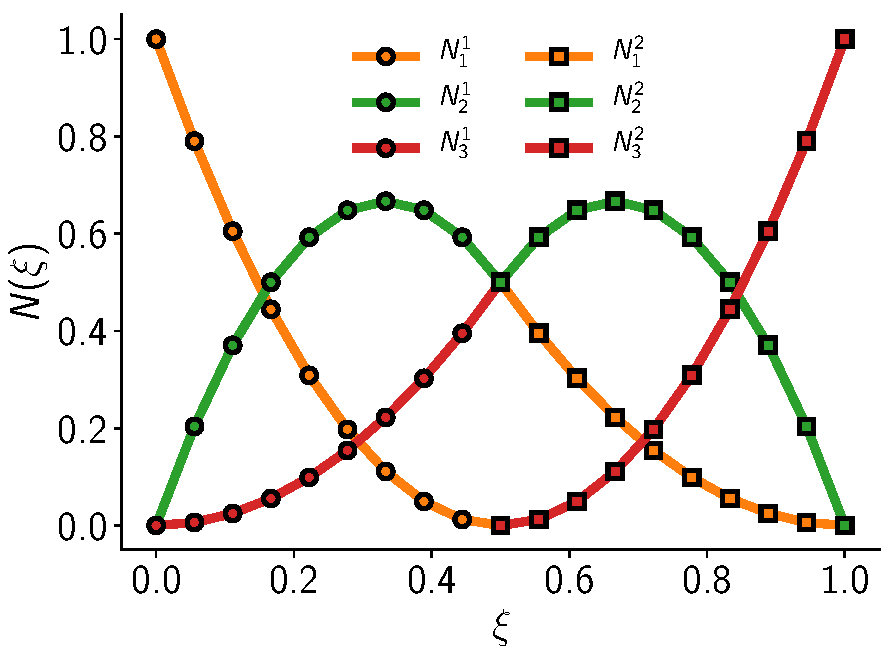
\includegraphics[width=1.0\textwidth]{figures/bar-basis-functions.pdf} \\
    \centering \footnotesize{shapes}
  \end{minipage}
  \begin{minipage}[b]{0.48\linewidth}
    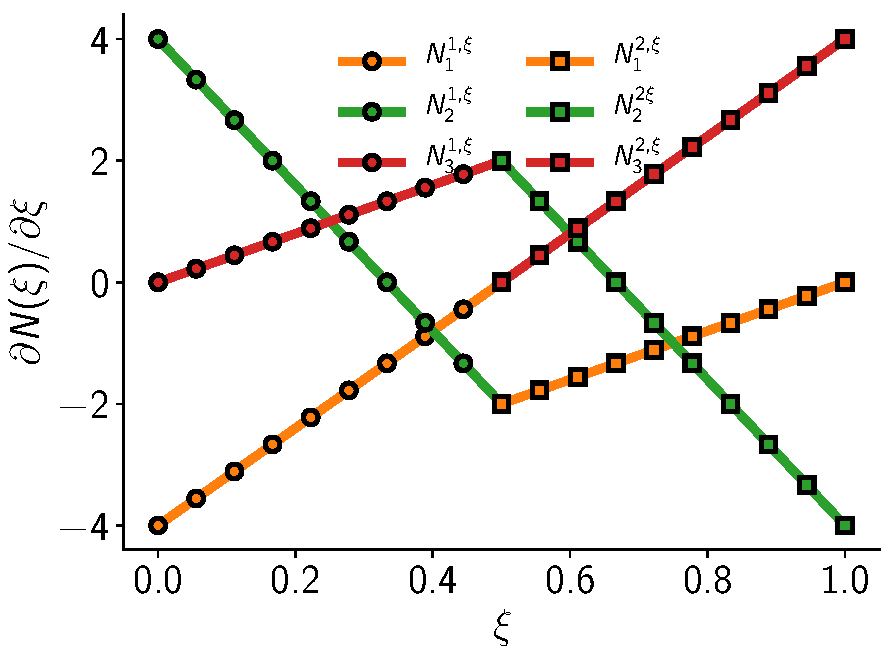
\includegraphics[width=1.0\textwidth]{figures/bar-basis-function-derivatives.pdf} \\
    \centering \footnotesize{derivatives}
  \end{minipage}
  \begin{equation}\nonumber
    \begin{aligned}
       & \textcolor{blue}{\text{element 1 [0,0.5]}}  & & \textcolor{blue}{\text{element 2 [0.5,1]}} \\
      N_1^1(\xi) &=  (2 \xi -1)^2 & N_1^2(\xi) &= (2\xi-2)(\xi-1)  \\
      N_2^1(\xi) &= -2\xi(3\xi-2) &N_2^2(\xi) &= -6\xi^2 + 8\xi -2 \\
      N_3^1(\xi) &=  2\xi^2       & N_3^2(\xi) &= (2\xi -1)^2 \\
    \end{aligned}
  \end{equation}
  % \end{block}


  \newpage



\end{frame}

%%%%%%%%%%%%%%%%%%%%%%%%%%%%%%%%%%%%%%%%%%%%%%%%%%%%%%%%%%%%%%%%%%%%%%
% Analysis of plate
%%%%%%%%%%%%%%%%%%%%%%%%%%%%%%%%%%%%%%%%%%%%%%%%%%%%%%%%%%%%%%%%%%%%%%

\section{Isogeometric Analysis of 2D-Plate}
    \begin{figure}
    \begin{center}
    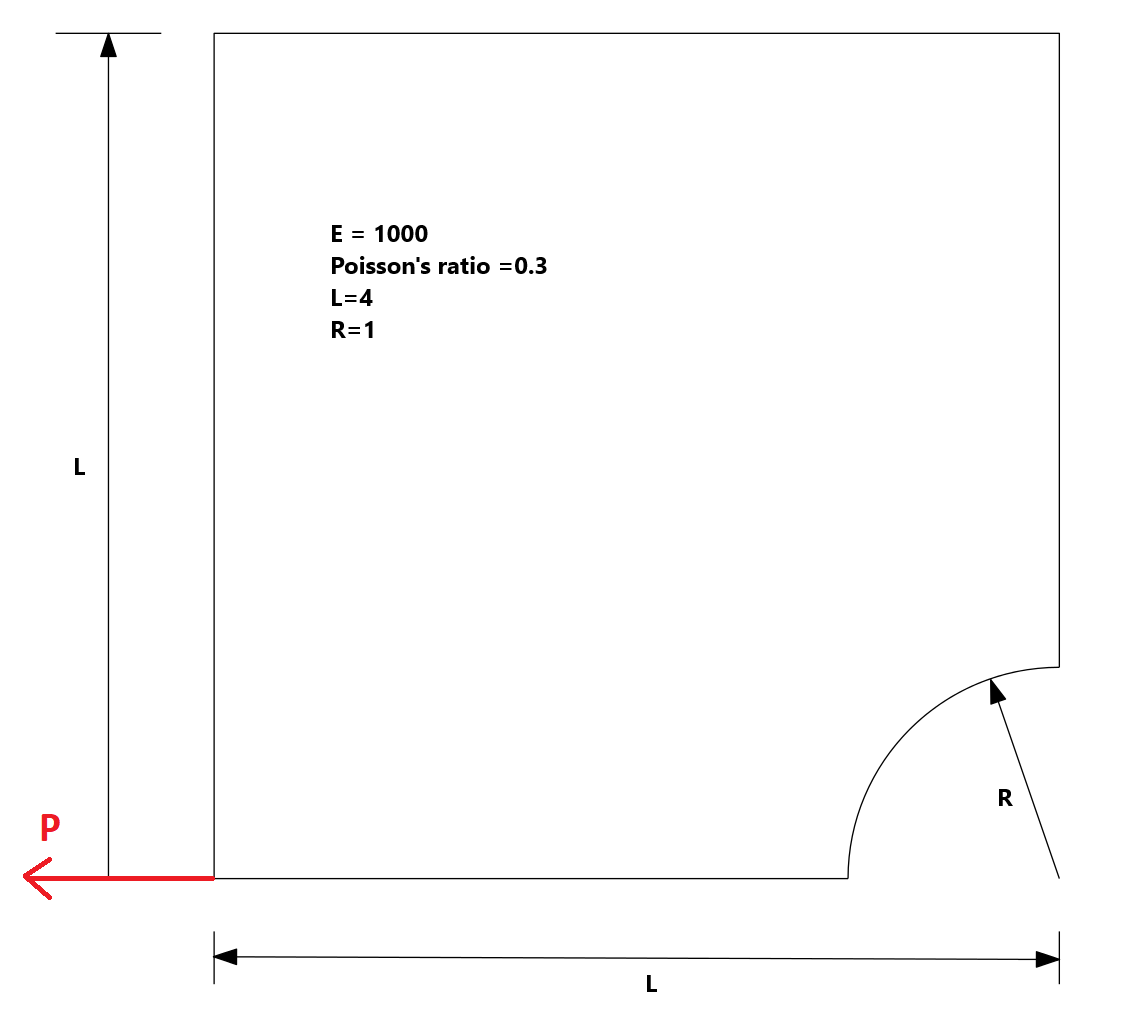
\includegraphics[width=4cm]{figures/plate2.png}
    \end{center}
    \caption{A plate with a hole}\label{Plate}
\end{figure}
  \begin{itemize}
    \item A plate of L=8 and W=8 with a circular hole is subjected to in-plane concentrated load.

    \item The geometry can be simplified to a quarter plate due to its symmetry as shown in Fig. \ref{Plate}. It is modeled using NURBS with 12 control points.

  \end{itemize}
  \newpage
  \begin{itemize}
    \item Divided the geometry into 2 elements and obtained connectivity arrays.
    \item Evaluated the NURBS basis function and its derivatives for all the gauss integration points to obtain strain displacement matrix.
    \begin{equation*}
        B=\begin{bmatrix}
        R_{1,x} & 0 & R_{2,x} & 0 & \dots & R_{9,x} & 0\\
        0 & R_{1,y} & 0 &R_{2,y} & \dots & 0 & R_{9,y}\\
        R_{1,y} & 0 &R_{1,x} &  R_{2,y} & \dots &  R_{9,y} &R_{9,x}
        \end{bmatrix}
    \end{equation*}
    \item B matrix is then used evaluate the element stiffness and force matrix and tr
    \begin{equation*}
        \int_{\Omega^e} (B^TCB  \,d\Omega)\,u = \int_{\Gamma^e_t} R.t \,d\Gamma +\int_{\Omega^e} R.f \,d\Omega
    \end{equation*}

    \item Assembled the element stiffness and force matrices into the global matrices using connectivity arrays.
    
  \end{itemize}
  \newpage
  \begin{minipage}[b]{0.48\linewidth}
    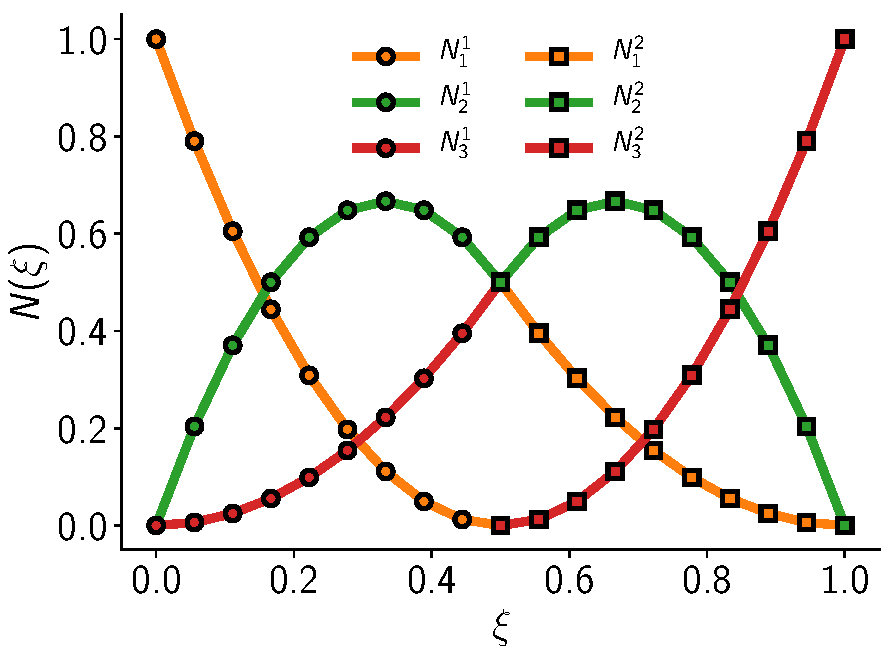
\includegraphics[width=1.0\textwidth]{figures/bar-basis-functions.pdf} \\
    \centering \footnotesize{shapes}
  \end{minipage}
  \begin{minipage}[b]{0.48\linewidth}
    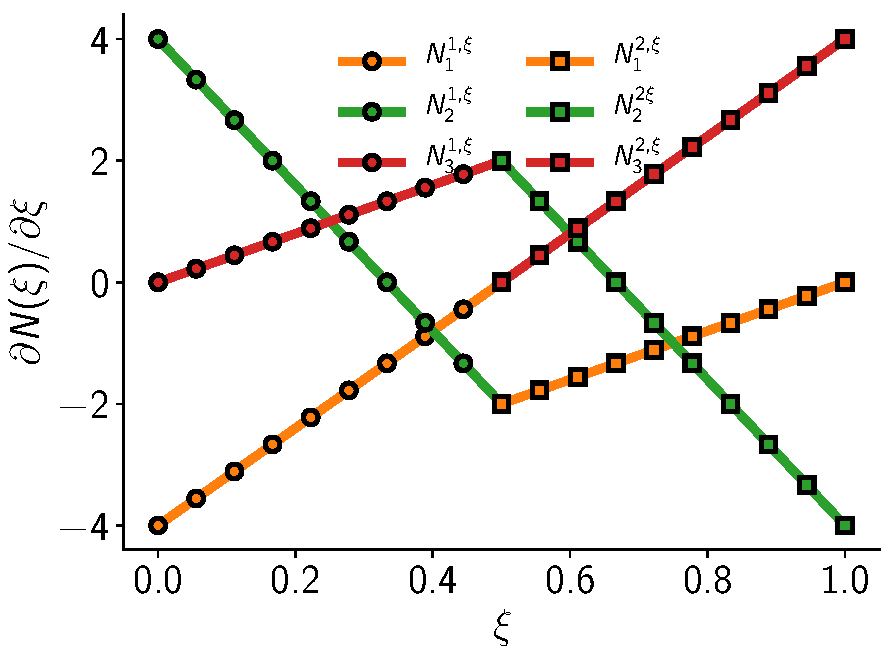
\includegraphics[width=1.0\textwidth]{figures/bar-basis-function-derivatives.pdf} \\
    \centering \footnotesize{derivatives}
  \end{minipage}
  \newpage
\end{frame}

%%%%%%%%%%%%%%%%%%%%%%%%%%%%%%%%%%%%%%%%%%%%%%%%%%%%%%%%%%%%%%%%%%%%%%
% Concluding remarks
%%%%%%%%%%%%%%%%%%%%%%%%%%%%%%%%%%%%%%%%%%%%%%%%%%%%%%%%%%%%%%%%%%%%%%

\section{Conclusions}
\begin{frame}[allowframebreaks] \frametitle{Conclusions}
  content
  \newpage
  content
  \newpage
\end{frame}

%%%%%%%%%%%%%%%%%%%%%%%%%%%%%%%%%%%%%%%%%%%%%%%%%%%%%%%%%%%%%%%%%%%%%%
% References and question
%%%%%%%%%%%%%%%%%%%%%%%%%%%%%%%%%%%%%%%%%%%%%%%%%%%%%%%%%%%%%%%%%%%%%%

\begin{frame}
  
  \begin{itemize}
  \item
  \item 
  \end{itemize}

  % git repo link
  
  \begin{columns}
    \column{6cm}
    \begin{block}{\centering{\huge  Any Questions?}}
      \centerline{ 
        
\includegraphics[width=0.5\textwidth]{figures/questions.png} 
      }
    \end{block}
  \end{columns}
  
\end{frame}

\end{document}







\section{Introduction and Motivation}


\begin{frame}[allowframebreaks]

  \frametitle{Introduction and Motivation}

\begin{itemize}

\item Computational methods have been playing an increasingly important role in science and engineering
analysis and design over the last several decades

\item In spite of the rapid advances and acceptance of numerical simulations, serious deficiencies 
remain in terms of accuracy, uncertainty, and validation for many applications

\item Uncertainty analysis is important since high fidelity computations typically 
assume perfect knowledge of all parameters. In reality there is much uncertainty due to
\begin{itemize}
\item manufacturing tolerances
\item in-service wear-and-tear
\item approximate modeling parameters
\end{itemize}

\newpage

\item Use of surrogate models for both uncertainty quantification and global optimizations has become popular
\begin{itemize}
\item Replace expensive function evaluations with an approximate but inexpensive functional representation
\item Can be probed exhaustively for global optimization or uncertainty analysis
\end{itemize}

\item An efficient gradient evaluation method based on adjoint formulations has been adopted by the computational community over the last several decades

$\rightarrow$ Introduction of gradient information within surrogate models has also attracted attention

\newpage

\item An efficient Hessian evaluation method has been developed in our group and we try to utilize the Hessian and gradient information
to counteract the ``curse of dimensionality'':

\begin{itemize}

\item For a single output objective, the effort for computing the full gradient is typically comparable to the effort of computing the objective function itself

\item As the number of inputs, $M$, increases, using the output function and its derivative provides \mbox{$M+1$} pieces of information for roughly the cost of two function evaluations

\item Similarly, the Hessian provides \mbox{$M \cdot (M+1)/2$} pieces of information for roughly the cost of $M$ function evaluations

\end{itemize}

$\rightarrow$ One can reasonably expect to have to compute the output function overall far fewer times to obtain a good surrogate model when using gradient and Hessian information

\end{itemize}


\end{frame}


%%%%%%%%%%%%%%%%%%%%%%%%%%%%%%%%%%%%%%%%%%%%%%%%%%%%%%%%%%%%%%%%
%%%                   Kriging Surrogate Model                %%%
%%%%%%%%%%%%%%%%%%%%%%%%%%%%%%%%%%%%%%%%%%%%%%%%%%%%%%%%%%%%%%%%

\section{Kriging Surrogate Model}

\subsection{Efficient Calculation of the Hessian}


\begin{frame}[allowframebreaks]

  \frametitle{Calculation of the Hessian}

\begin{itemize}

\item The Hessian, once obtained, can make various applications more efficient:

\begin{itemize}

\item Optimization
\item Extrapolation
\item Uncertainty analysis
\item Surrogate modeling

\end{itemize}

\item The most widely used method of finite differencing to obtain the Hessian is sensitive to step-size 
selection and is computationally expensive

\item The concept of using automatic differentiation (AD) in combination with 
an adjoint method to calculate the Hessian was initially investigated by Taylor {\em et al.} (1997) and refined for a steady 
CFD code by Ghate and Giles (2007)


\end{itemize}

\newpage

Derive the Hessian of a steady functional of interest
\bed
f(D)=F(D,q(D)) \quad \textrm{subject to} \quad R(D,q(D))=0
\eed
The first derivative of $f$ is given by
\bed
\pf{f}{D_j} = \pd{F}{D_j}+\pd{F}{q}\pf{q}{D_j},
\eed
and the Hessian by
\bed
\pff{f}{D_j}{D_k} = \mathfrak{D}_{jk} F +\pd{F}{q}\pff{q}{D_j}{D_k},
\eed
where
\bed
\mathfrak{D}_{jk} F = \pdd{F}{D_j}{D_k} + \pdd{F}{D_j}{q} q_k + \pdd{F}{D_k}{q} q_j + \pdt{F}{q} q_j q_k.
\eed

\end{frame}


\begin{frame}[allowframebreaks]

  \frametitle{More Efficient Formulation using the Adjoint}

Differentiating the flow residual equation gives
\bed
\pd{R}{D_j} + \pd{R}{q}\pf{q}{D_j} = 0,
\eed
and differentiating again we obtain,
\bed
\mathfrak{D}_{jk} R + \pd{R}{q} \pff{q}{D_j}{D_k} = 0,
\eed
with \mbox{$\mathfrak{D}_{jk} R$} defined analogues to \mbox{$\mathfrak{D}_{jk} F$}
\bed
\mathfrak{D}_{jk} R = \pdd{R}{D_j}{D_k} + \pdd{R}{D_j}{q} q_k + \pdd{R}{D_k}{q} q_j + \pdt{R}{q} q_j q_k. 
\eed

Defining the flow adjoint problem as
\bed
\left( \pd{R}{q} \right)^T \psi = \left( \pd{F}{q} \right)^T
\eed
simplifies the equations to
\begin{block}{ }
\vspace{-0.4cm}
\bea
\pf{f}{D_j} &=& \pd{F}{D_j}-\psi^T \pd{R}{D_j} \nonumber \\
\pff{f}{D_j}{D_k} &=& \mathfrak{D}_{jk} F - \psi^T \mathfrak{D}_{jk} R \nonumber
\eea
\end{block}

\newpage

\begin{itemize}

\item In order to calculate the complicated derivatives arising from \mbox{$\mathfrak{D}_{jk} F$} and  \mbox{$\mathfrak{D}_{jk} R$}
we double differentiate the corresponding routines in forward mode using TAPENADE

\item The computational cost for calculating the Hessian is

\begin{itemize}
\item one nonlinear baseline solution for $q$ using the flow residual
\item one linear adjoint solution for $\psi$
\item $M$ linear solutions for \mbox{$q_j=\pf{q}{D_j}$}
\end{itemize}

\item  One can parallelize the adjoint solutions for $\psi$ and the $M$ linear solutions for \mbox{$q_j$} as $M+1$ processes

$\rightarrow$ Assuming no limitations in the number of processors available, one can obtain the Hessian at the same time one calculates the gradient

\end{itemize}


\end{frame}





\begin{frame}[allowframebreaks]

  \frametitle{Dynamic Sample Point Selection}

\begin{itemize}

\item We refine the building of the Kriging model by a dynamic sample point selection
rather than just picking a predetermined number of sample points randomly

\item Start by evaluating the function (gradient and Hessian) value at the center of the domain

\item Pick an additional amount of sample points via latin hypercube sampling and evaluate their function (gradient and Hessian)

\item Then repeat the following steps until convergence

\begin{enumerate}

\item Specify a set of test candidates via latin hypercube sampling

\item Construct a local function value for each test candidate, $D$, using ``Dutch Intrapolation'':
\begin{itemize}
\item The function values and available derivatives of neighboring sample points, \mbox{$D_i$}, are used to construct extrapolations
\vspace{-0.2cm}
\bed
{\cal T}^{n_e}(D,D_i)=\sum_{|k|\ge 0}^{|k| \le n_e}\frac{a_k^{n_e}}{k!}(D-D_i)^k \partial^k {\cal J}(D_i) \quad \textrm{with} \quad a_k^{n_e}=1-k/(n_e+1)
\eed
\vspace{-0.3cm}
\item The extrapolations from a sufficient amount of neighboring sample points are then weighted with a low-order interpolant
\item Polynomial order of the intrapolant is equal to the combined extrapolation and interpolation polynomial order
\begin{minipage}[b]{0.35\linewidth}
\includegraphics[width=1.0\textwidth]{../figures/Rosenbrock.pdf} 
\end{minipage}
\begin{minipage}[b]{0.6\linewidth}
{\tiny Rosenbrock function and Dutch Intrapolation using function, gradient, and Hessian information with quadratic interpolation}
\end{minipage}
\end{itemize}

\item Compare the global Kriging surrogate model function value predictions for the test candidates with the local Dutch Intrapolations

\item Add a user-specified number of test candidates with the worst discrepancy between the two to the set of sample points, only then evaluating the real function 
(gradient and Hessian)

\end{enumerate}

\item Possible stopping criteria:
\begin{itemize}
\item Worst discrepancy below a certain threshold
\item Reach a maximum amount of function (gradient and Hessian) evaluations
\end{itemize}
\item We also augment the selection process by geometric criteria (e.g. sample points should not be too close)

\end{itemize}


\end{frame}



\begin{frame}

  \frametitle{Dynamic Sample Point Selection (Alternative Idea)}

\begin{itemize}

\item Instead of generating test candidates randomly generate a mesh using a high-dimensional Delaunay triangulation

\item Then specify a set of test candidates geometrically (e.g. centers of the hyper-triangles and the midpoints of the edges)
\centerline{
\includegraphics[width=0.24\textwidth]{../figures/triangulation.pdf} }

\item One has to start with all the corners of the domain as initial points which scales with $2^M$ rather than $\binom{M+n_i}{M}=\frac{(M+n_i)!}{M!n_i!}$

\item The Delaunay triangulation becomes the bottleneck of this procedure for more than half a dozen or so inputs


\end{itemize}

\end{frame}


\subsection{Accuracy}


\begin{frame}

\frametitle{Accuracy of Kriging Surrogate Model}

Three analytic test functions on $[-2,2]^M$:
\begin{enumerate}
\item A multidimensional Cosine function: \\
$f_1(x_1,\ldots,x_M)=\cos(x_1 + \ldots + x_M)$
\item The multidimensional Runge function:\\
 $f_2(x_1,\ldots,x_M)=\frac{1}{1+x_1^2 + \ldots + x_M^2}$
\item The multidimensional Rosenbrock function: \\
$f_3(x_1,\ldots,x_M)=\sum_{i=1}^{M-1} \left[ (1-x_i)^2+100(x_{i+1}-x_i^2)^2\right]$
\end{enumerate}

\centering
\begin{minipage}[b]{0.32\linewidth}
  \includegraphics[width=1.0\textwidth]{../figures/Cosinecompplot.pdf} \\
  \centering \footnotesize{Cosine function}
\end{minipage}
\begin{minipage}[b]{0.32\linewidth}
  \includegraphics[width=1.0\textwidth]{../figures/Rungecompplot.pdf} \\
  \centering \footnotesize{Runge function}
\end{minipage}
\begin{minipage}[b]{0.32\linewidth}
  \includegraphics[width=1.0\textwidth]{../figures/Rosenbrockcompplot.pdf} \\
  \centering \footnotesize{Rosenbrock function}
\end{minipage}

\end{frame}


\begin{frame}

\begin{center}
\Large Root-mean square error (RMSE) in two dimensions

\large Sample points are either selected through latin hypercube sampling (dashed) or dynamic sampling (solid)
\end{center}

\centering
\begin{minipage}[b]{0.32\linewidth}
  \includegraphics[width=1.0\textwidth]{../figures/RMSEdim2fct1.pdf} \\
  \centering \footnotesize{Cosine function}
\end{minipage}
\begin{minipage}[b]{0.32\linewidth}
  \includegraphics[width=1.0\textwidth]{../figures/RMSEdim2fct2.pdf}\\
  \centering \footnotesize{Runge function}
\end{minipage}
\begin{minipage}[b]{0.32\linewidth}
  \includegraphics[width=1.0\textwidth]{../figures/RMSEdim2fct3.pdf}\\
  \centering \footnotesize{Rosenbrock function}
\end{minipage}

\end{frame}


\begin{frame}

\begin{center}
\Large Root-mean square error (RMSE) in five dimensions

\large Sample points are either selected through latin hypercube sampling (dashed) or dynamic sampling (solid)
\end{center}

\centering
\begin{minipage}[b]{0.32\linewidth}
  \includegraphics[width=1.0\textwidth]{../figures/RMSEdim5fct1.pdf}\\
  \centering \footnotesize{Cosine function}
\end{minipage}
\begin{minipage}[b]{0.32\linewidth}
  \includegraphics[width=1.0\textwidth]{../figures/RMSEdim5fct2.pdf}\\ 
  \centering \footnotesize{Runge function}
\end{minipage}
\begin{minipage}[b]{0.32\linewidth}
  \includegraphics[width=1.0\textwidth]{../figures/RMSEdim5fct3.pdf}\\
  \centering \footnotesize{Rosenbrock function}
\end{minipage}

\end{frame}

%%%%%%%%%%%%%%%%%%%%%%%%%%%%%%%%%%%%%%%%%%%%%%%%%%%%%%%%%%%%%%%%
%%%                 Uncertainty Quantification               %%%
%%%%%%%%%%%%%%%%%%%%%%%%%%%%%%%%%%%%%%%%%%%%%%%%%%%%%%%%%%%%%%%%


\section{Uncertainty Quantification}

\begin{frame}[allowframebreaks]

  \frametitle{Uncertainty Analysis}

\begin{itemize}

\item Probabilistic assessment of uncertainty consists of three major phases:
\begin{enumerate}
\item characterization of input parameter variability from observations and physical evidence
\item propagation of input variabilities through the mathematical model
\item calculation of statistical properties of output
\end{enumerate}

\item Easiest and most accurate method for propagating aleatory uncertainties through the model
is a full nonlinear Monte Carlo (MC) simulation which is prohibitively expensive for
high fidelity computations

\newpage

\item If one is only interested in the mean and variance, moment methods can be a good choice

\item Moment methods are based on Taylor series expansions of the original non-linear objective function \mbox{${\cal J}(D)$}
about the mean of the input \mbox{$\mu_D$} given standard deviations \mbox{$\sigma_{D_j}$}

\item The resulting mean \mbox{$\mu_{\cal J}$} and variance \mbox{$\textrm{Var}_{\cal J}$} of the objective function are given to first order (\mbox{MM1}) by
\bea
\mu^{(1)}_{\cal J} &=&  {\cal J}(\mu_D) \nonumber\\
\textrm{Var}^{(1)}_{\cal J} &=&  \sum_{j=1}^{M} \left( \left. \pf{\cal J}{D_j} \right|_{\mu_D} \!\! \sigma_{D_j} \right)^2, \nonumber
\eea
and to second order (\mbox{MM2}) by
\bea
\mu^{(2)}_{\cal J}  \!\!\! &=&  \!\!\! \mu^{(1)}_{\cal J} + \half \sum_{j=1}^{M} \left( \left. \pft{\cal J}{D_j} \right|_{\mu_D} \!\! \sigma^2_{D_j} \right) \nonumber \\
\textrm{Var}^{(2)}_{\cal J}  \!\!\! &=&   \!\!\!  \textrm{Var}^{(1)}_{\cal J} + \half \sum_{j=1}^{M} \sum_{k=1}^{M} \left( \left. \pff{\cal J}{D_j}{D_k} \right|_{\mu_D} \!\! \sigma_{D_j} \sigma_{D_k} \right)^2. \nonumber
\eea

\item Note the non-linear shift between the mean of the output and the output of the mean is accounted for by the Hessian diagonal elements

\newpage

\item Extrapolation can be used for an inexpensive Monte Carlo (IMC) simulation with the advantage of being much cheaper than a full
non-linear MC simulation while still being able to obtain an approximate probability density function

\item Linear extrapolation (\mbox{Lin})
\begin{equation*}
{\cal J}_{\mbox{\tiny Lin}}(D)={\cal J}\Big(\mu_D\Big)+\left.\pf{{\cal J}}{D}\right |_{\mu_D} \!\!\!\!\! \cdot (D-\mu_D)
\end{equation*}

\item Quadratic extrapolation (\mbox{Quad}) 
\begin{equation*}
{\cal J}_{\mbox{\tiny Quad}}(D)={\cal J}_{\mbox{\tiny Lin}}(D) + \frac{1}{2} \left. \pft{{\cal J}}{D}\right |_{\mu_D} \!\!\!\!\! \cdot (D-\mu_D)^2
\end{equation*}

\newpage

\item For epistemic uncertainties MC methods can be employed as well, but the results can only be interpreted
with regards to the interval produced on the output functional

\item Other approaches, such as Dempster-Shafer evidence theory also require large numbers of function evaluations

\end{itemize}

\begin{block}{Claim}
\centering
The construction of an accurate surrogate model is one of the most effective options for propagating
both aleatory and epistemic uncertainties through a high fidelity simulation
\end{block}

\end{frame}









\subsection{Analytic Test Functions}



\begin{frame}

\frametitle{Analytic Test Functions}


\begin{center}
\Large Comparison of mean and variance predictions in 2D\\
\large $50,000$ normally distributed sample points\\
\large with \mbox{$\mu_D=(0,0)$} and \mbox{$\sigma_{D_1}=\sigma_{D_2}=0.6$}
\end{center}


\centering
\begin{tabular}{c|cc|cc|cc}
\hline
\hline
& \multicolumn{2}{c|}{Cosine fct} &  \multicolumn{2}{c|}{Runge fct} & \multicolumn{2}{c}{Rosenbrock fct} \\
\hline
& \footnotesize{Mean} & \footnotesize{Variance}  & \footnotesize{Mean} & \footnotesize{Variance} & \footnotesize{Mean} & \footnotesize{Variance}\\
\hline 
\footnotesize{Real} & \footnotesize{$0.697$} & \footnotesize{$0.133$} & \footnotesize{$0.658$} & \footnotesize{$4.11 \times 10^{-2}$} & \footnotesize{$76.19$} & \footnotesize{$2.51 \times 10^{4}$}  \\
\footnotesize{MM1} & \footnotesize{$1.0$} & \footnotesize{$0.0$}      & \footnotesize{$1.0$} & \footnotesize{$0.0$}                  & \footnotesize{$1.0$} & \footnotesize{$1.44$}\\
\footnotesize{Lin} & \footnotesize{$1.0$} & \footnotesize{$0.0$}      & \footnotesize{$1.0$} & \footnotesize{$0.0$}                  & \footnotesize{$1.0$} & \footnotesize{$1.44$} \\
\footnotesize{MM2} & \footnotesize{$0.640$} & \footnotesize{$0.259$} & \footnotesize{$0.280$} & \footnotesize{$5.18 \times 10^{-1}$}  & \footnotesize{$37.36$} & \footnotesize{$2.59 \times 10^{3}$} \\
\footnotesize{Quad} & \footnotesize{$0.639$} & \footnotesize{$0.259$} & \footnotesize{$0.280$} & \footnotesize{$5.19 \times 10^{-1}$} & \footnotesize{$37.36$} & \footnotesize{$2.59 \times 10^{3}$}  \\
\hline
\hline
\end{tabular}


\end{frame}


\begin{frame}

\begin{center}
\Large Error in the mean and variance predictions in 2D

\Large using the Kriging surrogate model 
\end{center}

\centering
\begin{minipage}[b]{0.32\linewidth}
  \includegraphics[width=1.0\textwidth]{../figures/Statserrordim2fct1.pdf}\\ 
  \centering \footnotesize{Cosine function}
\end{minipage}
\begin{minipage}[b]{0.32\linewidth}
  \includegraphics[width=1.0\textwidth]{../figures/Statserrordim2fct2.pdf} \\
  \centering \footnotesize{Runge function}
\end{minipage}
\begin{minipage}[b]{0.32\linewidth}
  \includegraphics[width=1.0\textwidth]{../figures/Statserrordim2fct3.pdf}\\ 
  \centering \footnotesize{Rosenbrock function}
\end{minipage}

\end{frame}


\begin{frame}

\begin{center}
\Large Comparison of mean and variance predictions in 5D \\
\large $50,000$ normally distributed sample points\\
\large with \mbox{$\mu_D=0$} and \mbox{$\sigma_{D_j}=0.6$}
\end{center}


\centering
\begin{tabular}{c|cc|cc|cc}
\hline
\hline
& \multicolumn{2}{c|}{Cosine fct} &  \multicolumn{2}{c|}{Runge fct} & \multicolumn{2}{c}{Rosenbrock fct} \\
\hline
& \footnotesize{Mean} & \footnotesize{Variance}  & \footnotesize{Mean} & \footnotesize{Variance} & \footnotesize{Mean} & \footnotesize{Variance}\\
\hline
\footnotesize{Real} & \footnotesize{$0.407$} & \footnotesize{$0.349$} & \footnotesize{$0.413$} & \footnotesize{$2.42 \times 10^{-2}$}  & \footnotesize{$304.6$} & \footnotesize{$1.32 \times 10^{5}$}  \\
\footnotesize{MM1} & \footnotesize{$1.0$} & \footnotesize{$0.0$}      & \footnotesize{$1.0$} & \footnotesize{$0.0$}                    & \footnotesize{$4.0$} & \footnotesize{$5.76$}\\
\footnotesize{Lin} & \footnotesize{$1.0$} & \footnotesize{$0.0$}      & \footnotesize{$1.0$} & \footnotesize{$0.0$}                    & \footnotesize{$4.0$} & \footnotesize{$5.77$} \\
\footnotesize{MM2} & \footnotesize{$0.1$} & \footnotesize{$1.62$}     & \footnotesize{$-0.8$} & \footnotesize{$1.30$}                  & \footnotesize{$149.4$} & \footnotesize{$1.05 \times 10^{4}$} \\
\footnotesize{Quad} & \footnotesize{$0.101$} & \footnotesize{$1.60$}  & \footnotesize{$-0.80$} & \footnotesize{$1.29$}                 & \footnotesize{$149.4$} & \footnotesize{$1.05 \times 10^{4}$}  \\ 
\hline
\hline
\end{tabular}


\end{frame}


\begin{frame}

\begin{center}
\Large Error in the mean and variance predictions in 5D

\Large using the Kriging surrogate model
\end{center}

\centering
\begin{minipage}[b]{0.32\linewidth}
  \includegraphics[width=1.0\textwidth]{../figures/Statserrordim5fct1.pdf}\\
  \centering \footnotesize{Cosine function}
\end{minipage}
\begin{minipage}[b]{0.32\linewidth}
  \includegraphics[width=1.0\textwidth]{../figures/Statserrordim5fct2.pdf}\\
  \centering \footnotesize{Runge function}
\end{minipage}
\begin{minipage}[b]{0.32\linewidth}
  \includegraphics[width=1.0\textwidth]{../figures/Statserrordim5fct3.pdf} \\
  \centering \footnotesize{Rosenbrock function}
\end{minipage}

\end{frame}






\subsection{Robustness Analysis of a Transonic Airfoil}

\begin{frame}[allowframebreaks]

  \frametitle{Robustness Analysis of a Transonic Airfoil}

\begin{itemize}

\item Consider steady inviscid case of transonic NACA 0012 airfoil

\item \mbox{$M_\infty=0.755$} with angle of attack of \mbox{$1.25^{\circ}$}

\item Computational mesh has about \mbox{$20,000$} triangular elements

\item Finite volume flow solver second-order in space and time \centerline{
\includegraphics[angle=-90,width=0.75\textwidth]{../figures/Contour}}

\item Robustness analysis of the lift coefficient $C_l$

\item Vary three shape design variable on the upper and three on the lower surface which control the magnitude of Hicks-Henne sine bump functions

\item Deformation of mesh via linear tension spring analogy

\item Assume same normal distributions for design variables with \mbox{$\mu_D=0$} and different standard deviations (shown are \mbox{$\pm 0.005$})

\centerline{ 
\includegraphics[width=0.85\textwidth]{../figures/Uncertainshapes}
} 

\item Stratified sampling with a sample size of $3,000$ is used

\end{itemize}

\end{frame}


\begin{frame}

\begin{center}
\large Mean and Variance of $C_l$ versus standard deviations
\end{center}
\vspace{-0.2cm}
\centerline{ 
\includegraphics[width=0.83\textwidth]{../figures/Robustnessplot} 
}


\end{frame}





%%%%%%%%%%%%%%%%%%%%%%%%%%%%%%%%%%%%%%%%%%%%%%%%%%%%%%%%%%%%%%%%
%%%              Conclusion and Future Work                  %%%
%%%%%%%%%%%%%%%%%%%%%%%%%%%%%%%%%%%%%%%%%%%%%%%%%%%%%%%%%%%%%%%%

\section{Conclusion and Future Work}

\begin{frame}

  \frametitle{Conclusion}

\begin{itemize}

\item Presented a gradient and Hessian enhanced Kriging surrogate model 

\item Augmented the model with dynamic sample point selection

\item Demonstrated the quality of the surrogate by comparison with higher-dimensional analytic test functions

\item Applied the surrogate to uncertainty quantification involving 
\begin{itemize}
\item Analytic test functions
\item Robustness analysis of a transonic airfoil
\end{itemize}

\end{itemize}

\end{frame}


\begin{frame}

  \frametitle{Future Work}


\begin{block}{Goal}
Develop a generic uncertainty quantification strategy which can 
call black-box simulation codes and makes use of gradient and Hessian information when available
\end{block}


\begin{itemize}

\item Speed up the construction of the Kriging model
\item Implement feature to calculate gradient and Hessian information only in important sample points
\item Investigate reduced Hessian and Hessian-vector product formulations
\item Perform epistemic uncertainty quantifications
\item Solve optimization under uncertainty problems 

(both robust and reliability designs) 

\end{itemize}


\end{frame}




\begin{frame}


\begin{columns}
\column{6cm}
\begin{block}{\centering{\huge  Any Questions?}}
\centerline{ 
\includegraphics[width=0.5\textwidth]{../figures/Question.jpg} 
}
\end{block}
\end{columns}

\end{frame}




%%%%%%%%%%%%%%%%%%%%%%%%%%%%%%%%%%%%%%%%%%%%%%%%%%%%%%%%%%%%%%%%
%%%                     End Document                         %%%
%%%%%%%%%%%%%%%%%%%%%%%%%%%%%%%%%%%%%%%%%%%%%%%%%%%%%%%%%%%%%%%%
\end{document}


